\documentclass[a4paper,11pt,fleqn]{article}%fleqn pour aligner les equations à gauche
\usepackage{graphicx}
\usepackage[utf8]{inputenc}  
\usepackage[T1]{fontenc}
\usepackage{lscape}

\usepackage{tgheros,textcomp}%Police Arial
\renewcommand{\familydefault}{\sfdefault}

%\setlength{\mathindent}{0pt}%indentation dans math = 0

\usepackage[top = 1cm, bottom = 2cm, left = 1cm, right = 1cm]{geometry}
\usepackage{titlesec}
%\setcounter{secnumdepth}{4}
\usepackage{xcolor}
\usepackage{amssymb} %double flèche de réaction
\usepackage{mathrsfs}%farraday
\usepackage{xtab}%tableau sur plusieurs pages
\usepackage{esvect}%grands vecteurs

\usepackage[version=4]{mhchem} %equations chimiques

\usepackage{array}
\usepackage{chemfig}
\usepackage{multirow}
%\usepackage{sectsty}

\usepackage{caption}
\usepackage{adjustbox}
\usepackage[labelformat=simple]{subfig}
\usepackage{float}


\usepackage{amsmath}
\usepackage{amssymb}
\usepackage[cal=boondoxo]{mathalfa} 
\usepackage{enumitem}
\usepackage{lastpage}
\usepackage{tcolorbox}
\usepackage{siunitx}
\usepackage[european, straightvoltages, RPvoltages]{circuitikz}
\usepackage{tikz}
\usetikzlibrary{shapes.geometric}
\usetikzlibrary{calc}
\usetikzlibrary{automata,positioning}
\usepackage{multicol}
\usepackage{eqnarray}
\usepackage{tabularx,colortbl}%colorer fond cellules

\sisetup{
	detect-all,
	output-decimal-marker={,},
	group-minimum-digits = 3,
	group-separator={~},
	number-unit-separator={~},
	inter-unit-product={~}
} %setup pour SIunitx

\usepackage{listings}%pour insérer le code python
\definecolor{codegreen}{rgb}{0,0.6,0}
\definecolor{codegray}{rgb}{0.5,0.5,0.5}
\definecolor{codepurple}{rgb}{0.58,0,0.82}
\definecolor{backcolour}{rgb}{0.95,0.95,0.92}


%\graphicspath{ {/home/rweye/Documents/Enseignement/2023/Cours/TSPE/Eval/Ressources/} }

\titleformat{\section}
{\titlerule
\vspace{.8ex}%
\normalfont \bfseries}
{\thesection :}{.5em}{\bfseries}

\renewcommand{\thesection}{Exercice \arabic{section}}
\titlespacing{\section}{0pt}{1em}{1em}
\renewcommand{\thesubsection}{\hspace{1cm}\alph{subsection}.}
\renewcommand\thesubfigure{\textbf{Document \arabic{subfigure} :}}

\title{\vspace{-1cm}\large 
	\begin{tabular}{|m{5cm}|>{\centering}m{8cm}|>{\centering\arraybackslash}m{4cm}|}
		\hline
		Nom : & \textbf{\textsc{DS TSPE N°1}} &  Note : \\
		Prénom : & & \\\hline
\end{tabular}}
\date{}

\newpagestyle{mystyle}{%
	\setfoot{ROSALIE}{\thepage\,$|$\,\pageref{LastPage}}{}
}
\renewpagestyle{plain}{%
	\setfoot{ROSALIE}{\thepage\,$|$\,\pageref{LastPage}}{}
}

\pagestyle{mystyle}

\newenvironment{itemize*}%
{\begin{itemize}[label=$-$]%
		\setlength{\itemsep}{0pt}%
		\setlength{\parskip}{0pt}}%
	{\end{itemize}}

\newenvironment{itemize**}%
{\begin{itemize}[label=,labelindent=0pt, leftmargin=*,topsep=0pt]%
		\setlength{\itemsep}{0pt}%
		\setlength{\parskip}{0pt}}%
	{\end{itemize}}

\renewcommand{\arraystretch}{1.5}


\begin{document}
\maketitle
\vspace{-2.5cm}

\section{Acides et bases dans la bouche}
	\subsection{L'émail}
	\begin{enumerate}
		\item Formule du phosphate de calcium solide : \ce{CaPO4(s)}
		\item L'oxygène neutre possède deux doublets liants et deux doublets non-liants autour de lui. Lorsqu'il porte une charge négative, l'oxygène possède un doublet liant et trois doublets non liants. Le schéma de Lewis de l'ion phosphate donne :\\
		
		\chemfig[atom sep =2em]{\charge{-135=\|,135=\|}{O}=P(-[:90]\charge{45:1.5pt=$\scriptstyle-$,180=\|,90=\|,0=\|}{O})(-[:-90]\charge{45:1.5pt=$\scriptstyle-$,-180=\|,-90=\|,0=\|}{O})=\charge{-45=\|,45=\|}{O}}
		\item Cet ion étant une base de Brönsted, son acide conjugué sera \ce{HPO4-}. On remarque que la molécule possède à la fois un H qu'elle est capable de céder un \ce{H+} et de capter un \ce{H+} grâce à son \ce{-O-}, elle est donc amphotère.
	\end{enumerate}
	
	\subsection{Les bactéries de la plaque dentaire}
	\begin{enumerate}[resume]
		\item Acide gluconique : \ce{C6H12O7}\\
		
		\chemfig[atom sep = 2em]{H-C(-[:-90]\charge{180=\|,0=\|}{O}-[:-90]H)(-[:90]H)-C(-[:-90]\charge{180=\|,0=\|}{O}-[:-90]H)(-[:90]H)-C(-[:-90]\charge{180=\|,0=\|}{O}-[:-90]H)(-[:90]H)-C(-[:-90]\charge{180=\|,0=\|}{O}-[:-90]H)(-[:90]H)-C(-[:-90]\charge{180=\|,0=\|}{O}-[:-90]H)(-[:90]H)-C(-[:-60]\charge{180=\|,-90=\|}{O}-H)=[:60]\charge{45=\|,135=\|}{O}}		 \\
		
		Acide lactique : \ce{C3H5O2}\\
		
		\chemfig[atom sep = 2em]{H-C(-[:-90]H)(-[:90]H)-C(-[:-90]\charge{180=\|,0=\|}{O}-[:-90]H)(-[:90]H)-C(-[:-60]\charge{180=\|,-90=\|}{O}-H)=[:60]\charge{45=\|,135=\|}{O}}
		\item L'acidité vient de la capacité d'une espèce chimique à céder un ou plusieurs ions \ce{H+}. Ici on observe que chacune de ces molécules possède un groupement acide carboxylique (\ce{R-COOH}) possédant une liaison \ce{O-H} polarisée à cause la forte différence d'électronégativité entre ces deux atomes. Ces deux molécules étant donc capables de céder un ion \ce{H+}, ce sont donc des acides de Brönsted.
		\item Ion gluconate : \ce{C6H11O7-} :\\
		
		\chemfig[atom sep = 2em]{H-C(-[:-90]O-[:-90]H)(-[:90]H)-C(-[:-90]O-[:-90]H)(-[:90]H)-C(-[:-90]O-[:-90]H)(-[:90]H)-C(-[:-90]O-[:-90]H)(-[:90]H)-C(-[:-60]\charge{45:1.5pt=$\scriptstyle-$,180=\|,-90=\|,0=\|}{O})=[:60]\charge{45=\|,135=\|}{O}}\\
		Ion lactate : \ce{C3H4O2-} :\\
		
		\chemfig[atom sep = 2em]{H-C(-[:-90]H)(-[:90]H)-C(-[:-90]\charge{180=\|,0=\|}{O}-[:-90]H)(-[:90]H)-C(-[:-60]\charge{45:1.5pt=$\scriptstyle-$,180=\|,-90=\|,0=\|}{O})=[:60]\charge{45=\|,135=\|}{O}}
		\item Réaction :  \ce{C3H5O2(aq) + PO4^{2-}(aq) -> C3H4O2-(aq) + HPO4-(aq)}\\
		On remarque ici que l'acide lactique réagit avec les ions phosphate qui constitue l'émail des dents. Cette réaction dissocie donc le phosphate des ions calcium. Il est donc possible d'imaginer que l'acide lactique participe à solubiliser les ions \ce{Ca^{2+}} et \ce{HPO4-} et donc créer des trous dans les dents.
		\item L'hydrogénocarbonate de sodium est une base faisant partie du couple : \ce{H2CO3(aq)} /\ce{HCO3-(aq)}. Elle peut donc réagit avec les acides contenus dans le milieu buccal pour limiter les attaques contre l'émail.
	\end{enumerate}
	
	\subsection{Érosion liée à l'alimentation}
	\begin{enumerate}[resume]
		\item Anne consomme 4 verres de 200 mL d'une solution de concentration $c_1$ = \SI{66}{\milli\mole\per\liter}. Elle consommera donc une quantité d'acide citrique valant : $$n_1 = c_1 \cdot V_{Anne}$$
		\noindent \fbox{AN :} $n_1 = \num{66E-3} \times 4\times \num{200E-3} = \SI{5.3E-2}{\mole}$\\
		Laure consomme 5 verres de 200 mL d'une solution de concentration $c_2$ = \SI{75}{\milli\mole\per\liter} d'acide malique doit une quantité de matière de :  $$n_2 = c_2 \cdot V_{Laure}$$
		\noindent \fbox{AN :} $n_2 = \num{75E-3} \times 5\times \num{200E-3} = \SI{7.5E-2}{\mole}$\\
		\item Le terme \emph{triacide} signifie que l'espèce chimique peut céder trois ions \ce{H+} tandis qu'un \emph{diacide} peut en céder deux.\\
		L'acide citrique est un triacide, il libèrera donc trois fois plus d'ions \ce{H+}, ce qui donne une quantité d'acide bue par Anne de \SI{1.6E-1}{\mole}\\
		Pour Laure, la quantité libérée par l'acide malique sera de  \SI{1.5E-1}{\mole}\\
		On retrouve des quantités relativement proche d'acide bus par les deux adolescentes, malgré les volumes et concentrations de départ différentes. Elles seront toutes deux sujettes au même niveau d'usure de l'émail.
	\end{enumerate}
	
	\subsection{Traitement de l'émail}
	\begin{enumerate}[resume]
		\item Réaction : \ce{H3PO4(aq) + PO4^{2-}(aq) ->  H2PO4-(aq) + HPO4-(aq)}
	\end{enumerate}
	
\section{La vanilline}
	\subsection{Synthèse de la vanilline}
	\begin{enumerate}
		\item On remarque dans la structure de la vanilline un groupement hydroxyle ainsi qu'un groupement carbonyle dont on peut retrouver les bandes caractéristiques, respectivement une bande large vers \SI{3200}{\per\centi\meter} et un pic intense vers \SI{1600}{\per\centi\meter}.\\ On notera la présence de nombreux pics entre \num{1000} et \SI{1500}{\per\centi\meter} correspondant aux liaisons d'un cycle portant une alternance de simples et doubles liaisons.
	\end{enumerate}
	
	\subsection{Principe du dosage de la vanilline}
	\begin{enumerate}[resume]
		\item On observe un pic d'absorbance vers \SI{345}{nm}, il se situe dans le domaine des ultra-violets et n'aura donc pas de couleur complémentaire dans le spectre visible. La solution d'ion phénolate sera donc incolore.
		\item On règlera l'appareil sur la valeur de $\lambda_{max}$ soit  \SI{345}{nm}
	\end{enumerate}
	
	\subsection{Dosage}
	\begin{enumerate}[resume]
		\item Courbe d'étalonnage :\\
		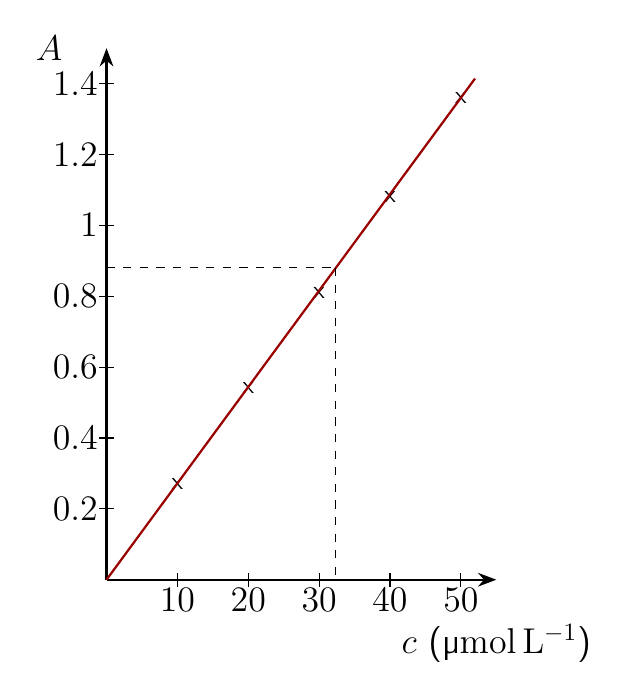
\begin{tikzpicture}[scale=.9,transform shape]
		\draw (5,13.6/2) node{x};
		\draw (4,10.8/2) node{x};
		\draw (3,8.1/2) node{x};
		\draw (2,5.4/2) node{x};
		\draw (1,2.7/2) node{x};
		\draw[thick, -Stealth] (0,0) to (5.5,0);
		\draw[thick, -Stealth] (0,0) to (0,7.5);
		\foreach \k in {1,...,5}{
		\pgfmathsetmacro{\lx}{\k*10}
			\draw (\k,-.1)--(\k,.1);
			\node[below] at (\k,0){\Large \pgfmathprintnumber[precision=1]{\lx}};
		}
		\foreach \k in {1,...,7}{
		\pgfmathsetmacro{\ly}{\k*0.2}
			\draw (-.1,\k)--(.1,\k);
			\node[left] at (0,\k){\Large \pgfmathprintnumber[precision=2]{\ly}};
		}
		\node[below] (c) at (5.5,-.5){\Large $c$ (\unit{\micro\mole\per\liter})};
		\node[left] (A) at (-.5,7.5){\Large $A$};
		
		\draw[thick,red!60!black, domain = 0:5.2]  plot (\x, 1.36*\x);
		
		\draw[dashed] (0,8.8/2)--(3.23,8.8/2);
		\draw[dashed] (3.23,8.8/2)--(3.23,0);
		
		\end{tikzpicture}
		\item La courbe d'étalonnage est une fonction linéaire, la relation de Beer-Lambert, impliquant une proportionnalité entre absorbance et concentration est bien respectée.
		\item Par lecture graphique on peut déterminer la concentration de la solution d'ion phénolate $c_{\ce{A-}}$ = \SI{32.3}{\micro\mole\per\liter}.\\
		La concentration de vanilline correspond à cette concentration d'ions phénolate.
		\item Le volume initial d'arôme de vanille utilisé est de \SI{1}{mL}. Il a été par la suite été dilué pour obtenir un volume de \SI{250}{mL} ce qui donne un facteur de dilution $F = \dfrac{V_f}{V_m} = \dfrac{\SI{250}{mL}}{\SI{1}{mL}} = 250$\\
		La concentration de la solution commerciale est donc 250 fois plus importante que celle détermine à la question précédente soit $c_{commerciale}$  = \SI{8.08E-3}{\mole\per\liter}\\
		La concentration en masse s'obtient par la relation $$ C_m = c \cdot M$$
		\fbox{AN :} $C_m = \num{8.08E-3} \times \num{152} = \SI{1.23}{\gram\per\liter}$\\
		On obtient donc $C_m$ = \SI{1.23}{\gram\per\liter}
	\end{enumerate} 
\end{document}